% This is samplepaper.tex, a sample chapter demonstrating the
% LLNCS macro package for Springer Computer Science proceedings;
% Version 2.20 of 2017/10/04
%
\documentclass[runningheads]{llncs}
%
\usepackage{graphicx}
\usepackage{enumitem}
\usepackage{xcolor}
% Used for displaying a sample figure. If possible, figure files should
% be included in EPS format.
%
% If you use the hyperref package, please uncomment the following line
% to display URLs in blue roman font according to Springer's eBook style:
% \renewcommand\UrlFont{\color{blue}\rmfamily}

\begin{document}
%
\title{Analiza operatiilor asociate unor structuri de date: Dictionar}
%
%\titlerunning{Abbreviated paper title}
% If the paper title is too long for the running head, you can set
% an abbreviated paper title here
%
\author{Vlad-Stefan Dieaconu} 
%
% First names are abbreviated in the running head.
% If there are more than two authors, 'et al.' is used.
%
\institute{Grupa 321CA, Facultatea de Automatica si Calculatoare \newline
Universitatea Politehnica Bucuresti \\
\email{vladstefandieaconu@gmail.com}\\}
%
\maketitle              % typeset the header of the contribution
%
\begin{abstract}
Aceasta lucrare isi propune analizarea principalelor structuri de date folosite in implementarea unui dictionar prin evidentierea avantajelor, cat si dezavantajelor, folosirii fiecareia dintre acestea.

\keywords{structuri de date  \and hash table \and arbori de cautare.}
\end{abstract}
%
%
%
\section{Introducere}

\subsection{Descrierea problemei rezolvate}
\quad  In viata de zi cu zi, ne confruntam cu procesul de stocarea ordonata a datelor, pentru a ne putea fi usor accesibile atunci cand avem nevoie de acestea. In acest sens, vom folosi structuri de date, ce sunt niste implementari particulare ale unor tipuri de date abstracte, acestea avand asociate o serie de operatii(algoritmi).

Apare astfel necesitatea definirii unei functii f : A $\rightarrow$ B, care primeste drept input un element a $\in$ A si returneaza˘ un element b $\in$ B, aceasta functie avand astfel rolul de a  realiza o mapare intre elementele celor doua multimi.

Acesta este, de altfel, modalitatea prin care definim notiunea de \textbf{dictionar}, ce realizeaza, in practica, o mapare intre cuvinte si definitiile acestora. 

\begin{figure}[ht!]
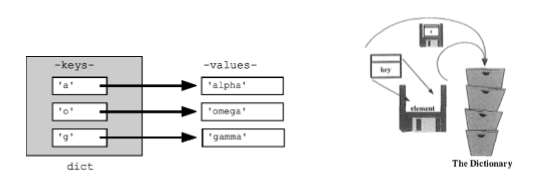
\includegraphics[width=90mm]{1.PNG}
\caption{Ilustrarea modului de functionare al unui dictionar \label{overflow}}
\end{figure}

Dictionarul este o structura de date abstracta, alcatuita dintr-o colectie de chei si valori, fiecarei chei fiindu-i asociata o valoare. Un dictionar poate fi implementat in diverse moduri, fiecare dintre aceste modalitati avand avantajele si dezavantajele ei, dupa cum voi demonstra pe parcursul acestei lucrari. 

\subsection{Exemple de aplicatii practice pentru problema aleasa}
Dictionarul isi gaseste aplicabilitatea in rezolvarea unor probleme precum spell-checking-ul sau oferirea de sugestii de catre un motor de cautare, in domeniul securitatii, in cazul aplicatiilor criptografice si a aplicatiilor ce rezolva probleme precum stocarea parolelor. De asemenea, acestea pot fi folosite, in industrie, pentru compresia si decompresia datelor.

\subsection{Specificarea solutiilor alese}
\quad Un \textbf{HashTable} este o structura de date eficienta pentru implementarea unui dictionar, intrucat timpul mediu de cautare al unui element este O(1), acesta generalizand notiunea simpla a unui array obisnuit. Cu toate acestea, un HashTable nu pastreaza o ordine atunci cand introduce cheile in dictionar, atingand performanta maxima pentru chei introduse aleatoriu. Din acest motiv, daca ordinea este importanta, trebuie sa ne indreptam atentia asupra altei metode de implementare, anume folosind arbori binari de cautare, cum sunt \textbf{arborii AVL}, pe care ii voi discuta in aceasta lucrare.

\subsection{Specificarea criteriilor de evaluare alese pentru validarea solutiilor}
\quad Pentru a testa corectitudinea, eficenta si performanta algoritmilor alesi, am realizat un generator, ce construieste teste cu input-uri aleatorii, in vederea testarii operatiilor specifice unui dictionar: insert(key, value), search(key), update(key, value), remove(key). Utilizatorul are posibilitatea de a alege dimensiunea datelor de intrare pentru fiecare operatie, atunci cand foloseste generatorul pentru a construi fisiere de input. 

Exista mai multe tipuri de teste, acestea fiind impartite in doua mari categorii: teste de acceptanta si teste de eficienta / performanta.

In cazul testelor de acceptanta ne intereseaza sa testam daca structura de date este corect implementata. Facem acest lucru efectuand o serie de operatii, ce ar trebui sa acopere toate cazurile posibile,  dupa care verificam daca rezultatul este cel la care ne-am asteptat, interogand dictionarul si comparand rezultatele cu cele corecte.

Pe de alta parte, dupa ce stim ca structura noastra de date este implementata corect, putem sa testam ii testam performanta, comparand implementarea noastra cu alte implementari, pentru a vedea care este cea mai rapida pentru anumite input-uri, in particular pentru cazul cel mai defavorabil al implementarii.

\section{Prezentarea solutiilor}

\subsection{Descrierea modului in care functioneaza algoritmii alesi}

Indiferent de tipul de implementare ales, asupra unui dictionar avem nevoie sa putem aplica urmatoarele operatii: 
\begin{itemize}
\item \textbf{get(key):} ce verifica daca dictionarul contine cheia \textbf{key} si returneaza elementul corespunzator acesteia, altfel returnand un element de tip null sau un constructor.
\vspace{\baselineskip}
\item \textbf{put(key, value):} ce are rolul de a insera o noua pereche in dictionar.
\vspace{\baselineskip}
\item \textbf{update(key, value):} care verifica daca in dictionar exista deja un element avand respectiva cheie, caz in care ii modifica valoarea cu una noua.
\vspace{\baselineskip}
\item \textbf{remove(key):} ce verifica daca dictionarul contine cheia key, caz in care elimina perechea corespunzatoare respectivei chei.
\end{itemize}
\vspace{\baselineskip}

\textbf{HASHTABLE}-ul este, in general, implementat prin intermediul unui array, in care fiecare element poarta denumirea de bucket. Acesta se foloseste de o functie speciala, numita functie de hash, care transforma fiecare cheie primita, intorcand un indice al array-ului, purtand denumirea de valoare de hash a cheii.

\vspace{\baselineskip}
O functie de hash ideala este in mod simultan: 

$\bullet$ \textbf{universala} - poti sa introduci orice parametru de intrare

$\bullet$ \textbf{repetabila} - de fiecare data cand introduci variabila X vei obtine acelasi rezultat Y

$\bullet$ \textbf{unidirectionala} - este usor sa calculezi valoarea functiei pe baza variabilei introduse in functie (f(x) → x), dar imposibil sa afli variabila pe baza valorii funcţiei (x → f(x));

$\bullet$ \textbf{biunivoca} - ai garantia ca variabile diferite vor produce valori diferite ale funcţiei (unicitate) – dar şi viceversa, ai garantia că o valoare a functiei corespunde cu o singura variabilă posibila;

$\bullet$ \textbf{concisa} -  produce rezultate cu o marime predeterminata, indiferent de marimea variabilei de intrare.
\vspace{\baselineskip}

Intrucat suntem limitati din punct de vedere tehnologic, orice functie de hash va avea coliziuni, adica valori de input diferite (insemnand chei diferite), pentru care functia de hash produce acelasi output (valoarea de hash a celor doua chei este identica). Pentru ca existenta coliziunilor creste complexitatea temporala a algoritmilor, una dintre provocarile de care ne lovim este alegerea unei metode de tratare a acestor coliziuni. Exista mai multe metode de tratare a coliziunilor, cum este inlantuirea sau adresarea deschisa. 

\vspace{\baselineskip}
$\bullet$ \textbf{Inlantuirea} - aceasta modalitate de tratare a coliziunilor presupune implementarea dictionarului ca un array de array-uri. Elementele ce au aceeasi valoare de hash a cheii, dispersandu-se in acelasi loc, fiind retinute in acelasi array. 

\begin{figure}[ht!]

\includegraphics[width=120mm]{2.PNG}
\caption{Ilustrarea metodei de inlantuire \label{overflow}}
\end{figure}

Cazul cel mai defavorabil in cazul folosirii inlantuirii pentru tratarea coliziunilor este atunci cand toate cheile produc acelasi rezultat in urma aplicarii functiei de hash. Astfel, vom avea un array cu un singur element, reprezentat de un alt array cu n elemente. 
\vspace{\baselineskip}

$\bullet$ \textbf{Adresarea deschisa} - aceasta metoda de tratare a coliziunilor presupune memorarea tuturor elementelor in interiorul tabelei de dispersie, pe urmatoarea pozitie libera, pana cand aceata se umple complet, caz in care este redimensionata, folosind un factor de redimensionare (ce este in general egal cu 2). 
Cazul cel mai defavorabil este intalnit atunci cand table noastra este aproape plina (in teorie, acest lucru insemnand ca gradul de ocupare al tabelei este de peste 80$\%$), pentru ca in acest punct, cautarea urmatoarei pozitii libere din tabela devine foarte costisitoare. 

\vspace{\baselineskip}

O alta metoda de implementare a dictionarului este folosind \textbf{arbori binari de cautare}, acestia oferind propietatea ca, fata de hashtable-uri, pastreaza o ordine specifica a cheilor introduse. In particular, acestia au fost implementati folosind arborii AVL.

\textbf{Arborele AVL}-ul este un arbore binar de cautare echilibrat dupa inaltime, ce se reechilibreaza la fiecare operatie de adaugare sau stergere a unui element din dictionar. Diferenta intre doi subarbori ai oricarui nod este de maxim 1.
Cheile se afla in interiorul nodurilor, dupa cum se poate observa in Fig. 3.

\begin{figure}[ht!]
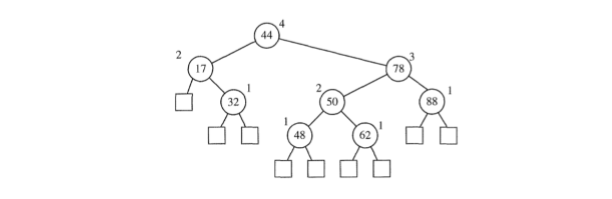
\includegraphics[width=150mm]{3.PNG}
\caption{Exemplu arbore AVL \label{overflow}}
\end{figure}

La inserare se adauga nodul astfel incat sa aiba proprietatea de arbore binar de cautare, iar dupa se verifica factorul de balansare si se incepe sau nu balansarea lui. Balansarea lui se face cu rotatii duble. Exista 4 tipuri de rotatii duble: \textbf{LL, LR, RL, RR}.

Se definesc astfel doua variabile, denumite factor de balans si invariant, calculate folosind urmatoarele formule (Fig. 4). 
\vspace{\baselineskip}

\begin{figure}[ht!]
\centering
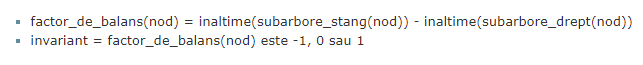
\includegraphics[width=120mm]{4.PNG}
\caption{Formule pentru invariant si factor de balansare \label{overflow}}
\end{figure}


Daca factorul de balans este pozitiv, iar factorul de balans al nodului stang este pozitiv, aplicam LL.

Daca factorul de balans este pozitiv, iar factorul de balans al nodului stang este negativ, aplicam LR.

Daca factorul de balans este negativ, iar factorul de balans al nodului drept este pozitiv, aplicam RL.

Daca factorul de balans este negativ, iar factorul de balans al nodului drept este negativ, aplicam RR.




\subsection{Analiza complexitatii solutiilor}
In cazul implementarii unui hashtable folosind inlantuirea pentru tratarea coliziunilor, avem urmatoarele complexitati pentru cazul mediu:

\begin{itemize}
\item \textbf{adaugarea unui element: \(\Theta(1)\) } 
\item \textbf{cautarea si stergerea unui element: \(\Theta(a)\)}, unde a este gradul de ocupare al tabelei de dispersie
\end{itemize}
\vspace{\baselineskip}

Pentru cazul cel mai nefavorabil, cand toate elementele introduse in dictionar au aceeasi valoare de hash a cheii, complexitatea este:

\begin{itemize}
\item \textbf{adaugarea unui element: O(1) }, intrucat pot pur si simplu sa pun un element la finalul bucketului. Daca este insa nevoie de verificarea existentei elementului in dictionar, complexitatea devine O(N)
\item \textbf{cautarea si stergerea unui element: O(N)}, unde N este numarul de elemente din lista.
\end{itemize}
\vspace{\baselineskip}


In cazul implementarii unui hashtable folosind adresarea directa, pentru cazul mediu, complexitatile sunt:

\begin{itemize}
\item \textbf{adaugarea, cautarea fara succes a datelor si stergerea unui element}: $\Theta$( \( \frac{1}{1 + a} \) ), unde a este gradul de ocupare al tabelei de dispersie, a = \( \frac{N}{M} \) , unde N este dimensiunea datelor, iar M este dimensiunea tabelei de dispersie folosite.

\item \textbf{cautarea cu succes a datelor} se realizeaza in $\Theta$( \( \frac{1}{a} \) ln ( \( \frac{1}{1-a} \) ) ), a fiind factorul de incarcare definit anterior
\end{itemize}
\vspace{\baselineskip}

Pentru cazul cel mai nefavorabil, cand factorul de umplere al tabelei este de peste 80$\%$, se prefera folosirea inlantuirii, intrucat complexitatea worst-case este O(N).
\vspace{\baselineskip}

In cazul arborilor binari de cautare complexitatea in cazul cel mai rau este de O(N), in particular, cand vorbim de arborii AVL, complexitatea in cazul cel mai defavorabil este de O(log N). Cazul cel mai nefavorabil este atunci cand, dupa o operatie de insert sau de delete, este necesar sa facem rotatii pentru fiecare nod. 

\begin{figure}[ht!]
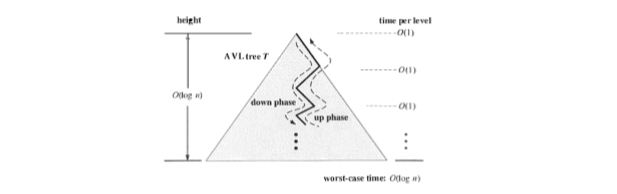
\includegraphics[width=150mm]{6.PNG}
\caption{Timpul de rulare in cazul operatiilor de search si modify intr-un AVL \label{overflow}}
\end{figure}



\subsection{Prezentarea principalelor avantaje si dezavantaje pentru solutiile luate in considerare}
\quad In functie de tipul operatiilor pe care le vom aplica dictionarului nostru, este posibil sa fie mai avantajos un mod de implementare fata de altul. 

Implementarea folosind un hashtable poate fi mai avantajoasa in unele cazuri, fiind o structura de date bune atunci cand avem de efectuat numeroase operatii de adaugare sau stergere, intrucat nu este necesara echilibrarea, ca in cazul AVL-ului. Daca dimensiunea datelor de intrare este cunoscuta, putem obtine performante foarte bune indiferent de operatiile efectuate, alegand bine functia de hash si dimensiunea initiala a tabelei de dispersie. Nu in ultimul rand, putem spune ca este o structura de date mai usor de inteles (si de implementat) fara de un arbore AVL. 

Principalul avantaj al folosirii arborilor binari de cautare este faptul ca ne permit sa tinem elementele intr-o anumita ordine, putand realiza de asemenea parcurgeri inordine, prin care sa obtinem elementele sortate crescator). In cazul in care avem nevoie, ne este usor sa obtinem cel mai mic sau cel mai mare element introdus in structura, aceasta fiind o propietate a arborilor binari de cautare. Nu in ultimul rand, in cazul arborilor binari de cautare, complexitatea (raportata la memoria totala utilizata de intreaga structura de date) este foarte buna, nefolosind mai mult spatiu decat are nevoie (fata de tabelele de dispersie, cand alocam un array de o dimensiune fixa, fara a stii daca il vom umple sau nu). 

In functie de modul in care alegem sa tratam coliziunile, putem avea avantaje sau dezavantaje aditionale in cadrul folosirii unui hashtable. Inlantuirea este preferata adresarii directe intrucat poate fi folosita cu succes cand dimensiunea datelor de intrare nu este cunoscuta si nu are nevoie de redimensionare deoarece foloseste liste, iar complexitatea operatiei de adaugare este mereu O(1). Pe de alta parte, adresarea deschisa este preferata inlantuirii in cazul in care cunoastem dimensiunea datelor de intrare, insa performanta hashtable-ului scade drastic atunci cand gradul de ocupare depaseste 80$\%$, dupa cum putem observa in Fig. 5.

\begin{figure}[ht!]
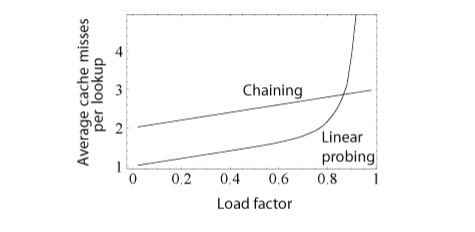
\includegraphics[width=150mm]{5.PNG}
\caption{Linear probing vs Chaining \label{overflow}}
\end{figure}



\section{Evaluare}
\subsection{Descrierea modalitatii de construire a setului de teste folosite pentru validare}
Am realizat un generator, ce genereaza teste cu input-uri random, dimensiunea datelor fiind aleasa de catre utilizator. Pentru validarea corectitudinii operatiilor, efectuez o serie de operatii de adaugare, stergere si modificare, urmand ca la final sa verific elementele continute in structura mea de date, pentru a vedea daca operatiile au fost realizate in mod corect. 

Pentru testarea eficentei in cazul mediu, iau input-uri random de diverse dimensiuni si compar timpii obtinuti pentru operatiile de inserare, modificare si stergere, pentru fiecare structura de date.

Pentru a testa cazul cel mai defavorabil, pentru dictionar am ales o functie de hash basic, ce genereaza foarte multe coliziuni, functia care intoarce ultima cifra a numarului primit parametru. 


\subsection{Mentionati specificatiile sistemului de calcul pe care ati rulat testele}
Testele au fost rulate pe un sistem avand urmatoarele specificatii:

Operating System: Windows 10 Education 64-bit 

Processor: Intel(R) Core(TM) i7-6700HQ CPU @ 2.60GHz (8 CPUs), ~2.6GHz

Memory: 8192MB RAM

Available OS Memory: 8012MB RAM

Page File: 6239MB used, 6637MB available

DirectX Version: DirectX 12

DxDiag Version: 10.00.17134.0001 64bit Unicode

\subsection{Ilustrarea, folosind grafice, a rezultatelor evaluarii solutiilor pe setul de teste}

\begin{figure}[ht!]
\centering
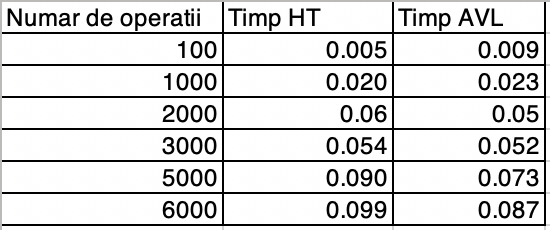
\includegraphics[width=80mm]{8.png}
\caption{HashTable VS AVL \label{overflow}}
\end{figure}

Fig. 8 prezinta timpul de executie per numarul de operatii pentru cele doua structuri de date analizate in aceasta lucrare, AVL si hashtable.

\begin{figure}[ht!]
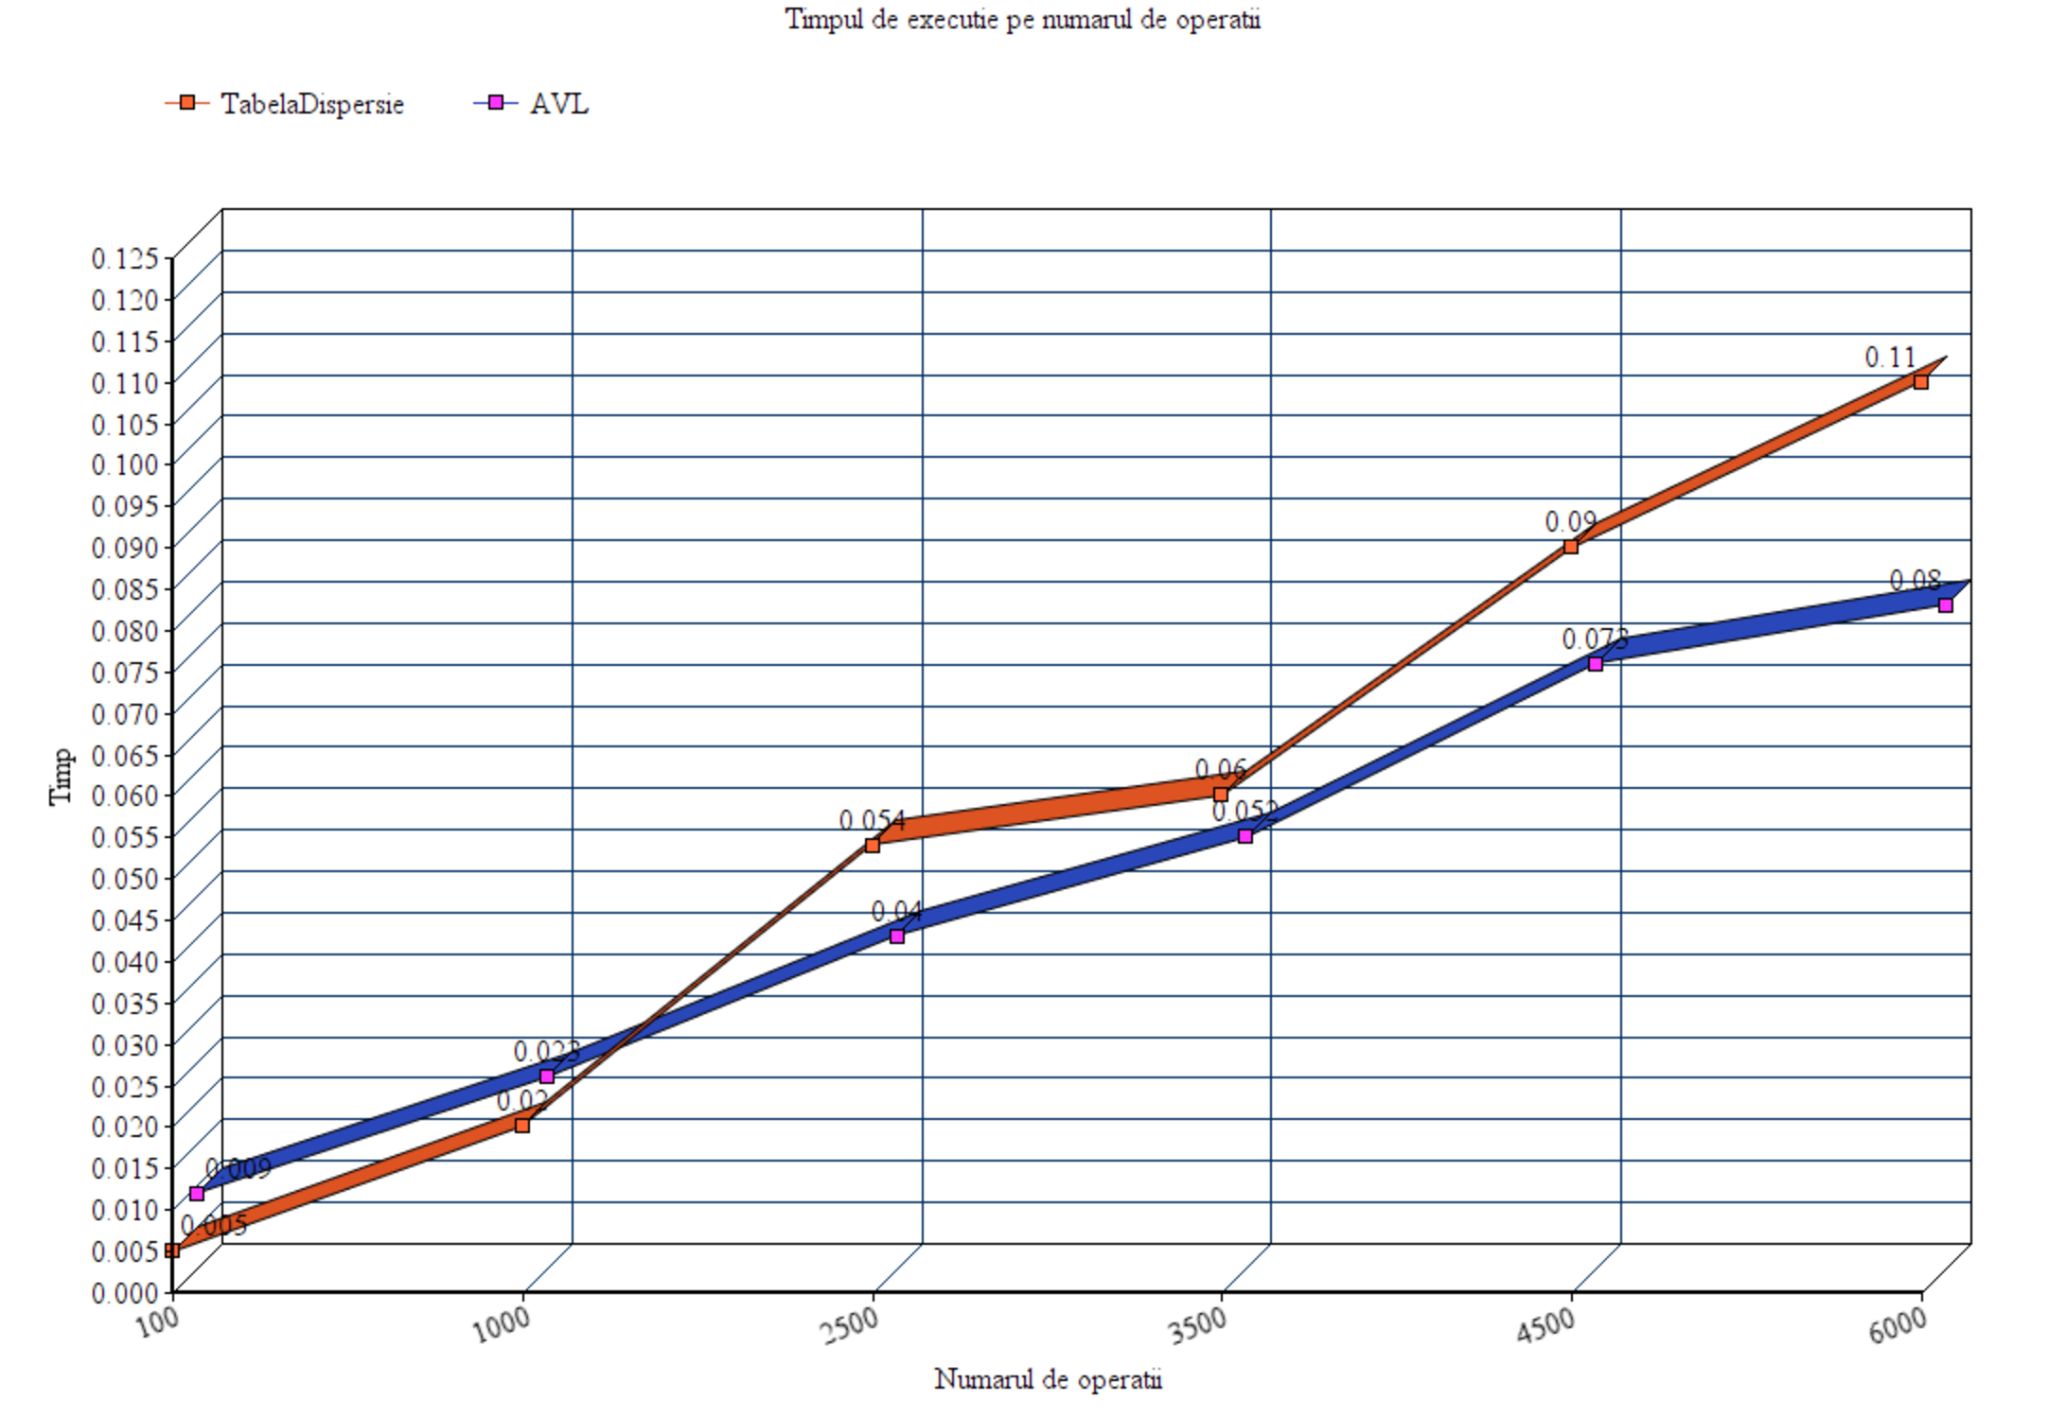
\includegraphics[width=150mm]{7.png}
\caption{HashTable VS AVL \label{overflow}}
\end{figure}

\subsection{Prezentarea valorilor obtinute pe teste}
Dupa cum se poate vedea, arborii AVL ofera un timp mai bun decat hashtable-ul, pentru date de intrare de dimensiuni mari. Trebuie insa sa avem in vedere ca input-urile sunt random, motiv pentru care alegerea unei functii de hash buna, care sa aiba cat mai putine coliziuni, poate fi dificila. Acest lucu reiese si din Fig 7, ce prezinta timpii obtinuti.



\section{Concluzii}
\subsection{Abordarea problemei in practica}
Dupa cum am spus, in cazul arborilor AVL, inserarile si stergerile pot fi foarte costisitoare, motiv pentru care este de preferat folosirea cand operatiile de cautare sunt foarte dese, iar inserarile foarte rare. O aplicatie practica ar fi folosirea in cazul unei aplicatii de tipul "Mersul trenurilor", intrucat foarte rar sunt adaugate rute noi, in schimb cautarea este foarte frecventa si lucram cu multe date (rute).

O aplicatie practica pentru implementarea folosind tabele de dispersie este, de pilda, in implementarea cache-urilor de pe site-urile de internet, unde vrem sa putem adauga cache-uri noi si sa le modificam de fiecare data cand intram pe un site. 


\begin{thebibliography}{8}
\bibitem{ref_article1}
Donald E. Knuth, The Art of Computer Programming, Volume Three/ Sorting and searching, Second Edition, 1998

\bibitem{ref_book1}
Collections \url{http://elf.cs.pub.ro/poo/laboratoare/colectii}.

\bibitem{ref_book1}
OCW: DATA STRUCTURES \url{https://ocw.cs.pub.ro/courses/sd-ca}.

\bibitem{ref_book1}
Thomas H. Cormen, Charles E. Leiserson, Ronald L. Rivest, Clifford Stein: INTRODUCTION TO ALGORITHMS, Third Edition: III Data Structures



\bibitem{ref_proc1}
GeeksForGeeks \url{https://www.geeksforgeeks.org/}
\end{thebibliography}
\end{document}
